\documentclass{article}
\usepackage{graphicx}% Required for inserting images
\usepackage{lindrew}
\usepackage{pdfpages}
\usepackage[shortlabels]{enumitem}
\usepackage{algorithm}
\usepackage{algpseudocode}

\title{ACM 104 Problem Set 1}
\author{Amitesh Anand Pandey}
\date{October 2024}
\begin{document}
\maketitle
\section*{Problem 1}
If $AB = C$, then from the problem statement we have
\begin{equation*}
    c_{ij} = \sum_{k = 1}^{p} a_{ik}b_{kj}
\end{equation*}
For any column $j$ of $C$, we have that
\begin{equation*}
    c_{j} = \sum_{k = 1}^{p}a_{k}b^{kj}
\end{equation*}
Then, since $C = [c_{1}, c_{2}, \dots, c_{n}]$, substituting the expressions for the columns we get
\begin{equation*}
    C = \left[\sum_{k = 1}^{p}a_{k}b^{k1}, \sum_{k = 1}^{p}a_{k}b^{k2}, \dots, \sum_{k = 1}^{p}a_{k}b^{kn}\right]
\end{equation*}
Since the summation for each column follows the same form, we can represent $C$ as follows:
\begin{equation*}
    C = \sum_{k = 1}^{p} \left[a_{k}b^{k1}, a_{k}b^{k2}, \dots , a_{k}b^{kn}\right]
\end{equation*}
By definition of matrix multiplication, we can now write
\begin{equation*}
    C = AB = \sum_{k=1}^{p}a_{k}b^{k}
\end{equation*}
\newpage
\section*{Problem 2}
(a) Notice that for $a, b \in \mathbb{R}$, we can rewrite the expression as
\begin{equation*}
    a^{-1} - b^{-1} = a^{-1}(b-a)b^{-1}
\end{equation*}
This leads us to the guess that for matrices, the identity is
\begin{equation*}
    A^{-1} - B^{-1} = A^{-1}(B-A)B^{-1}
\end{equation*}
To prove this, see that $A^{-1}(B-A)B^{-1} = (A^{-1}B - I)B^{-1} = (A^{-1}I - IB^{-1}) = A^{-1} - B^{-1}$ as desired. \\\\
\noindent{(b)} First, from the definition of the derivative, we have
\begin{equation*}
    \frac{\text{d}A^{-1}}{\text{d}t} = \lim_{\Delta t \to 0} \frac{(A+ \Delta A)^{-1} - A^{-1}}{\Delta t}
\end{equation*}
Upon employing the identity derived in 2(a), we obtain
\begin{equation*}
    \frac{\text{d}A^{-1}}{\text{d}t} = \lim_{\Delta t \to 0} \left[(A + \Delta A)^{-1} \left(-\frac{\Delta A}{\Delta t}\right)A^{-1}\right] 
\end{equation*}
Now as $\Delta t$ goes to $0$, trivially $\Delta A$ does too. The first coefficient becomes $A^{-1}$ itself, thus finally we have
\begin{equation*}
    \frac{\text{d} A^{-1}}{\text{d}t} = -A^{-1}A'(t)A^{-1}
\end{equation*}
For the special case where $A$ is a family of functions, recall that the inverse of a scalar output of a function can simply be written by $1/A(t)$. Thus, from the identity above we have
\begin{equation*}
    \frac{\text{d}}{\text{d}t}A^{-1}(t) = - \frac{1}{A(t)}\cdot A'(t) \cdot \frac{1}{A(t)} = -\frac{1}{A^{2}}A'(t)
\end{equation*}
On the other hand, from the power and chain rules for differentiation, we also have
\begin{equation*}
    \frac{\text{d}A^{-1}}{\text{d}t} = \frac{\text{d}A^{-1}}{\text{d}A}\cdot \frac{\text{d}A}{\text{d}t} = \frac{\text{d}}{\text{d}A}\left(\frac{1}{A(t)}\right)\cdot A'(t) = - \frac{1}{A^{2}}A'(t)
\end{equation*}
Thus our identity works for the special case of functions. \\\\
(c) To find an identity for the derivative of $A^{2}$ with respect to $t$, we once again begin with the definition of the derivative as follows:
\begin{equation*}
    \frac{\text{d}A^{2}}{\text{d}t} = \lim_{\Delta t \to 0} \frac{(A(t + \Delta t))^{2} - A(t)^{2}}{\Delta t}
\end{equation*}
For the sake of notational simplicity, assume that $\Delta t$ brings about a corresponding $\Delta A$ change in the matrix $A(t)$. So now let $A(t + \Delta t) = A(t) + \Delta A$. Note that since $A$ depends smoothly on $t$, we also have $A(t) + \Delta A \to A$ as $\Delta t \to 0$. Then replacing this expression in the derivative, we have
\begin{equation*}
    \frac{\text{d}A^{2}}{\text{d}t} = \lim_{\Delta t \to 0}\frac{(A+\Delta A)^{2} - A^{2}}{\Delta t} = \lim_{\Delta t \to 0}\frac{A^{2} + A\cdot \Delta A + \Delta A \cdot A + \Delta A^{2} - A^{2}}{\Delta t}
\end{equation*}
Since $\Delta A^{2}$ surely vanishes as $\Delta t \to 0$, we obtain
\begin{equation*}
    \frac{\text{d}A^{2}}{\text{d}t} = \lim_{\Delta t \to 0} A \frac{\Delta A}{\Delta t} + \frac{\Delta A}{\Delta t} A = AA'(t) + A'(t)A
\end{equation*}
\section*{Problem 3}
From running the code, we hypothesize that $P_{n} = I_{n}$, 
\begin{equation*}
l_{ij}=\left\{\begin{array}{lr}
(1-i)/i, & \text { for } i=j+1 \\
1, & \text { for } i=j \\
0, & \text { for elsewhere}
\end{array}\right.
\end{equation*}
\begin{equation*}
u_{ij}=\left\{\begin{array}{lr}
(j+1)/j, & \text { for } i=j \\
-1, & \text { for } i=j-1 \\
0, & \text { for elsewhere}
\end{array}\right.
\end{equation*}
The above rules indicate that $P, L, \text{and } U$ must follow the following patterns:
\begin{equation*}
    P = \begin{pmatrix}
        1 & 0 & \dots & 0\\
        0 & 1 & \ & \vdots \\
        \vdots & & \dots & \\
        0 & \dots & & 1
    \end{pmatrix}\text{, } L = \begin{pmatrix}
        1 & 0 & \dots & 0\\
        -\frac{1}{2} & 1 & \dots & 0 \\
        \vdots & -\frac{2}{3}& 1 & \vdots \\
        0 & \dots & \frac{1-n}{n} & 1
    \end{pmatrix}\text{, and } U = \begin{pmatrix}
        \frac{2}{1} & -1 & \dots & 0\\
        0 & \frac{3}{2} &  & \vdots\\
        \vdots & & \frac{4}{3} & -1\\
        0 &\dots & & \frac{n+1}{n}
        
    \end{pmatrix}
\end{equation*}
\noindent{Now}, we will proceed with the proof that the above described definitions of $P_{n}, L_{n}$ and $U_{n}$ satisfy $P_{n}A_{n} = L_{n}U_{n}$. 
\begin{proof}
    First note, if $P_{n} = I_{n}$, we have $P_{n}A_{n} = I_{n}A_{n} = A_{n}$. So we must show that $A_{n} = L_{n}U_{n}$. Let's try to find $L_{n}U_{n}$. Assume $B_{n} = L_{n}U_{n}$. Then we have
    \begin{equation*}
        b_{ij} = \sum_{k = 1}^{n}l_{ik}u_{kj}
    \end{equation*}
    Consider the follows cases encompassing all $b_{ij}$: 
    \begin{enumerate}
        \item When $i, j = 1$ (main diagonal), we have
        \begin{equation*}
            b_{11} = \sum_{k=1}^{n}l_{11}u_{11} = 2
        \end{equation*}
        \item When $i = j - 1$ (super diagonal), we have
        \begin{equation*}
            b_{ij} = \sum_{k=1}^{n}l_{ik}u_{kj} = -1
        \end{equation*}
        \item When $i = j,\text{ and }i, j \neq 1$ (main diagonal), we have
        \begin{equation*}
            b_{ij} = \sum_{k=1}^{n}l_{ik}u_{kj} = -\left(\frac{1-i}{i}\right) + \frac{j+1}{j} = \frac{2i}{i} = 2
        \end{equation*}
        \item When $i = j + 1$ (sub diagonal), we have
        \begin{equation*}
            b_{ij} = \left(\frac{1-i}{i}\right)\cdot\left(\frac{j+1}{j}\right) = -1
        \end{equation*}
        \item Finally, in all other cases, the sum only has `0' terms, thus $b_{ij} = 0$. 
    \end{enumerate}
    Now, note that Cases (1) and (3) ensure that $B_{n}$ has the same main diagonal as $A_{n}$. Cases (2) and (4) ensure that $B_{n}$ has the same super and sub diagonals as $A_{n}$. Case (5) ensures that $B_{n}$ has all other elements `0,' just like $A_{n}$. Thus the product matrix $B_{n} = A_{n}$.
\end{proof}
\section*{Problem 4}
(a) From the definition of an orthogonal matrix, we have that any $P \in \mathbb{M}_{n\times n}$ is orthogonal if $P^{T} = P^{-1}$. Now notice that this implies that $P$ is orthogonal if and only if $PP^{T} = PP^{-1} = I_{n}$. Thus it is sufficient to show that $PP^{T} = I_{n}$. 
\begin{equation*}
    (PP^{T})_{ij} = \sum_{k=1}^{n}p_{ik}p^{T}_{kj}
\end{equation*}
Now observe that $p^{T}_{kj} = p_{jk}$, so we have
\begin{equation*}
    (PP^{T})_{ij} = \sum_{k=1}^{n} p_{ik}p_{jk}
\end{equation*}
Intuitively, we can imagine that $(PP^{T})_{ij}$ is filled by iterating through all columns of both rows $i$ and $j$ and taking the sum of pair-wise products of corresponding cells in both of the rows. We know that a single column cannot have a repeat '1' in a permutation matrix, thus $(PP^{T})_{ij} = 1$ only when $i$ and $j$ are the same row, so that the `1' cell is multiplied by itself \emph{once}. Then this implies that
\begin{equation*}
(PP^{T})_{ij}=\left\{\begin{array}{lr}
1, & \text { when } i=j\\
0, & \text { everywhere else}
\end{array}\right.
\end{equation*}
This is exactly the definition of the identity matrix $I_{n}$. Thus $P^{T} = P^{-1}$ and $P$ is orthogonal.\\\\
\noindent{(b)}  We will prove that an orthogonal matrix need not be a permutation matrix by method of counterexample. Consider the matrix
\begin{equation*}
A = \begin{pmatrix}
    \frac{1}{\sqrt{2}} & \frac{1}{\sqrt{2}}\\
    \frac{1}{\sqrt{2}} & -\frac{1}{\sqrt{2}}
\end{pmatrix}
\end{equation*}
Obviously $A$ is not a permutation matrix since it contains values other than $0$ and $1$. Note that 
\begin{equation*}
    A^{T} = \begin{pmatrix}
    \frac{1}{\sqrt{2}} & \frac{1}{\sqrt{2}}\\
    \frac{1}{\sqrt{2}} & -\frac{1}{\sqrt{2}}
\end{pmatrix} = A
\end{equation*}
Since $A^{T} = A$, obviously $A^{T}A^{-1} = AA^{-1} = I$, thus $A$ is orthogonal but not permutational. 
\section*{Problem 5}
\begin{proof} We will have
\begin{equation*}
    A = \frac{1}{2}(A + A^{T}) + \frac{1}{2}(A - A^{T})
\end{equation*}
Now, we will show that $\frac{1}{2}(A + A^{T})$ is symmetric and that the matrix $\frac{1}{2}(A-A^{T})$ is skew-symmetric. Observe that
\begin{equation*}
    \frac{1}{2}(A+A^{T})_{ij} = \frac{1}{2}(A_{ij} + A^{T}_{ij}) = \frac{1}{2}(A^{T}_{ji} + A_{ji}) = \frac{1}{2}(A + A^{T})_{ji}
\end{equation*}
Thus $1/2(A+A^{T}) = 1/2(A+A^{T})^{T}$, thus the first term is symmetric. Now notice that
\begin{equation*}
    \frac{1}{2}(A-A^{T})_{ij} = \frac{1}{2}(A_{ij} - A^{T}_{ij}) = \frac{1}{2}(A^{T}_{ji} - A_{ji}) = -\frac{1}{2}(A - A^{T})_{ji}
\end{equation*}
Thus $1/2(A-A^{T}) = -1/2(A-A^{T})^{T}$ and the second term is skew symmetric. Hence, $A$, an arbitrary square matrix, can be expressed as a sum of appropriate symmetric and skew symmeteric matrices.
\end{proof}
\section*{Problem 6}
(a) Recall that the rank of a matrix is invariant of the elementary row operations applied to it. Thus, we will prove that the number of linearly independent rows spanning $B$ is 2, thereby proving $\text{rank}(B) = 2$ using a sequence of row operations as follows: $R_{k} : R_{k} - R_{k-1}$ for $1 < k \leq n$. Then we have
\begin{equation*}
    B' = \begin{pmatrix}
        1 & 2 & \dots & n\\
        n & n & \dots & n \\
        \vdots & \vdots & &\vdots \\
         n &  n & \dots & n
    \end{pmatrix}
\end{equation*}
Clearly that $R_{2},R_{3},\dots,R_{n}$ are all identical rows. Then it follows that we have only $2$ linearly independent rows spanning $B'$ (or $B$). So then the $\text{rank}(B) = 2$.\\
(b) \emph{Code attached in the end}, the non-zero elements of $x$ are $x_{99} = 1.37\cdot 10^{-14}$ and $x_{100} = 0.01$. 
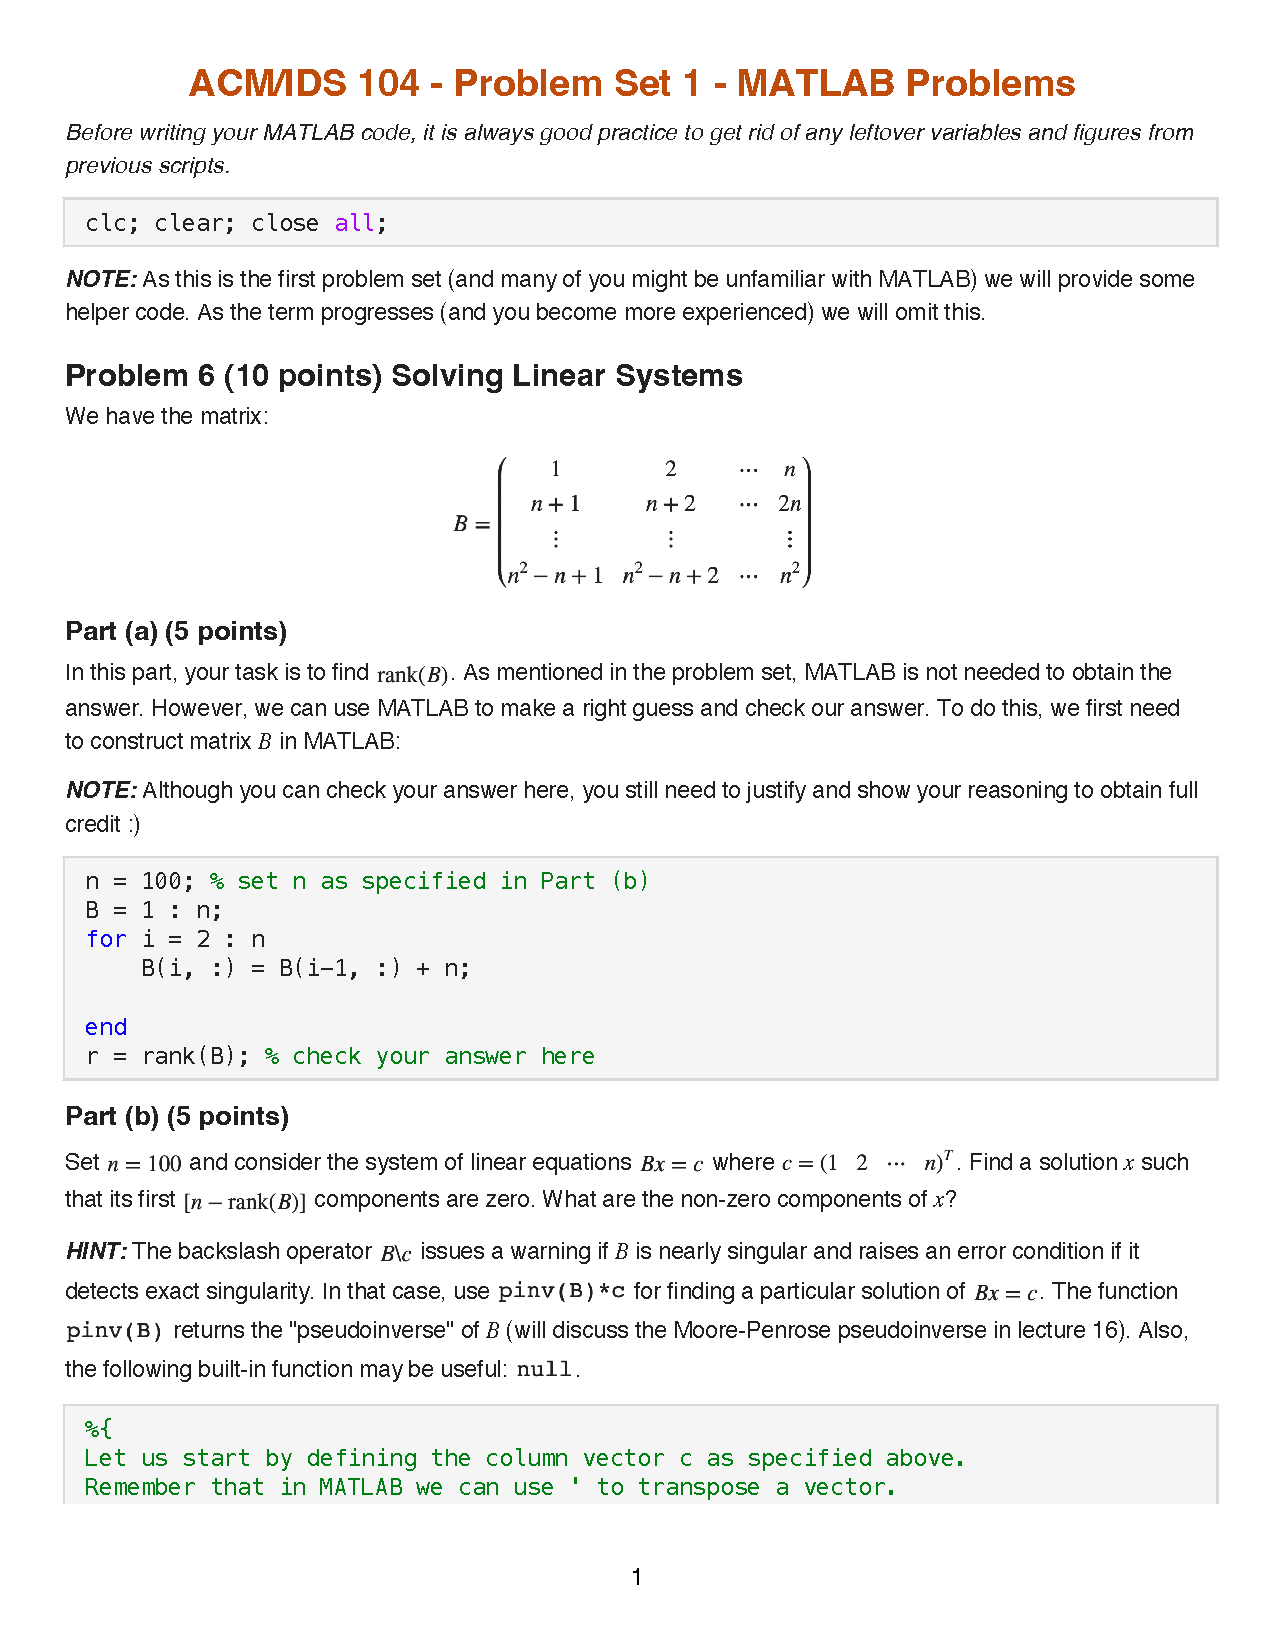
\includepdf[pages=-]{PS1completed.pdf}



\end{document}
